% Slides for 2025-02-24
% To create a slide, use the following:
% \begin{frame}{TITLE}
%     BODY
% \end{frame}

% To create a slide with a bullet list, use the following:
% \begin{frame}{TITLE}
%     \begin{itemize}
%         \item ITEM 1
%         \item ITEM 2
%     \end{itemize}    
% \end{frame}

% To create a slide with numbered list, use the following:
% \begin{frame}{TITLE}
%     \begin{enumerate}
%         \item ITEM 1
%         \item ITEM 2
%     \end{enumerate}
% \end{frame}

% To create a slide with a graphic:
% 1. Add the graphic to this folder (named picture.png)
% 2. Use the following:
% \begin{frame}{TITLE}
%     \centering
%     \includegraphics[height=0.7\textheight,width=0.7\textwidth,keepaspectratio]{picture.png}
% \end{frame}

% To create a slide with two columns, use the following:
% \begin{frame}{TITLE}
%     \begin{columns}
%         \begin{column}{0.5\textwidth}
%             COLUMN 1 BODY
%         \end{column}
%         \begin{column}{0.5\textwidth}
%             COLUMN 2 BODY
%         \end{column}
%     \end{columns}
% \end{frame}



\begin{frame}{TDOA Localization Investigation: Tower Placement}
    \begin{columns}
        \begin{column}{0.48\textwidth}
            \centering
            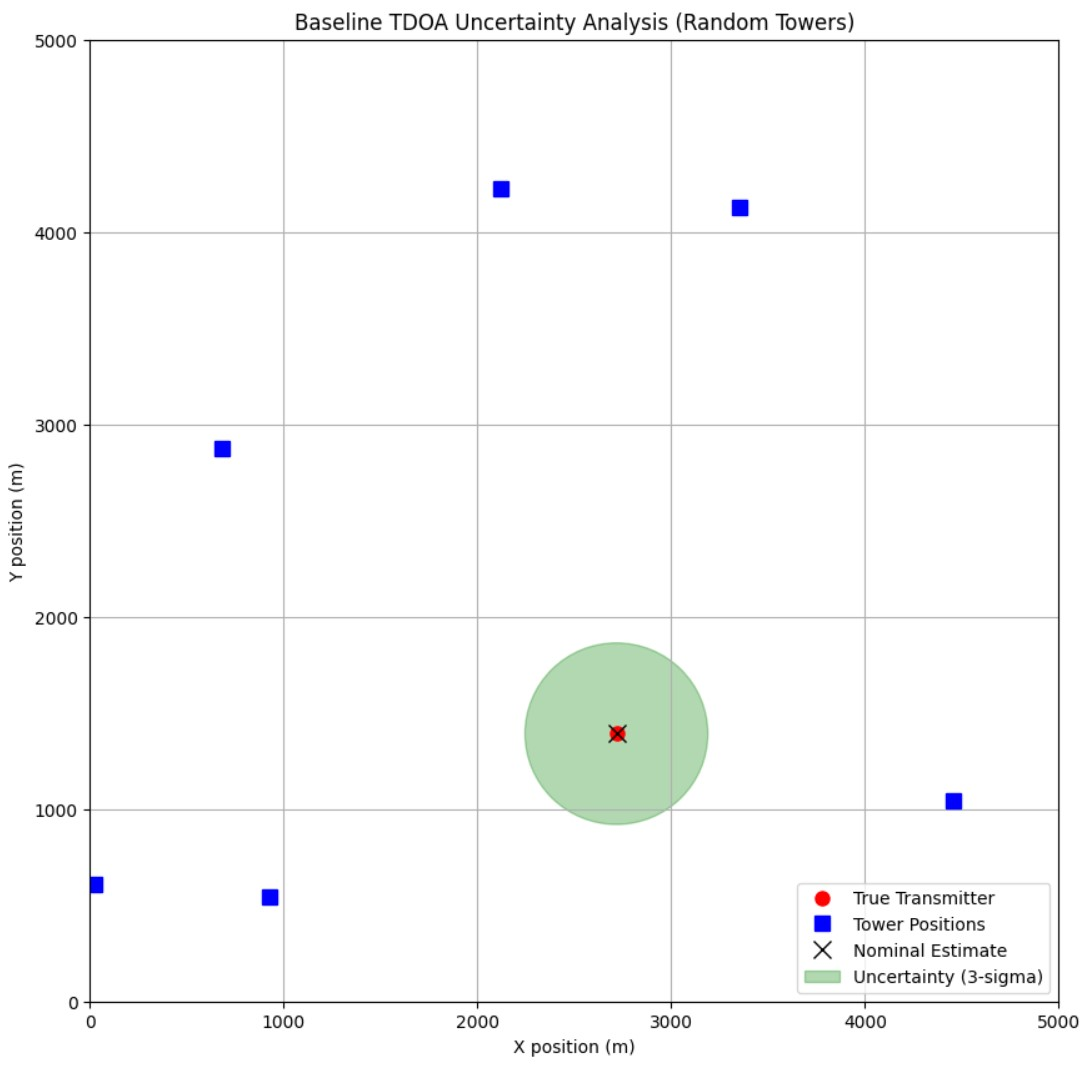
\includegraphics[width=\textwidth,keepaspectratio]{images/rtt/random_towers.jpg}
        \end{column}
        \begin{column}{0.48\textwidth}
            \centering
            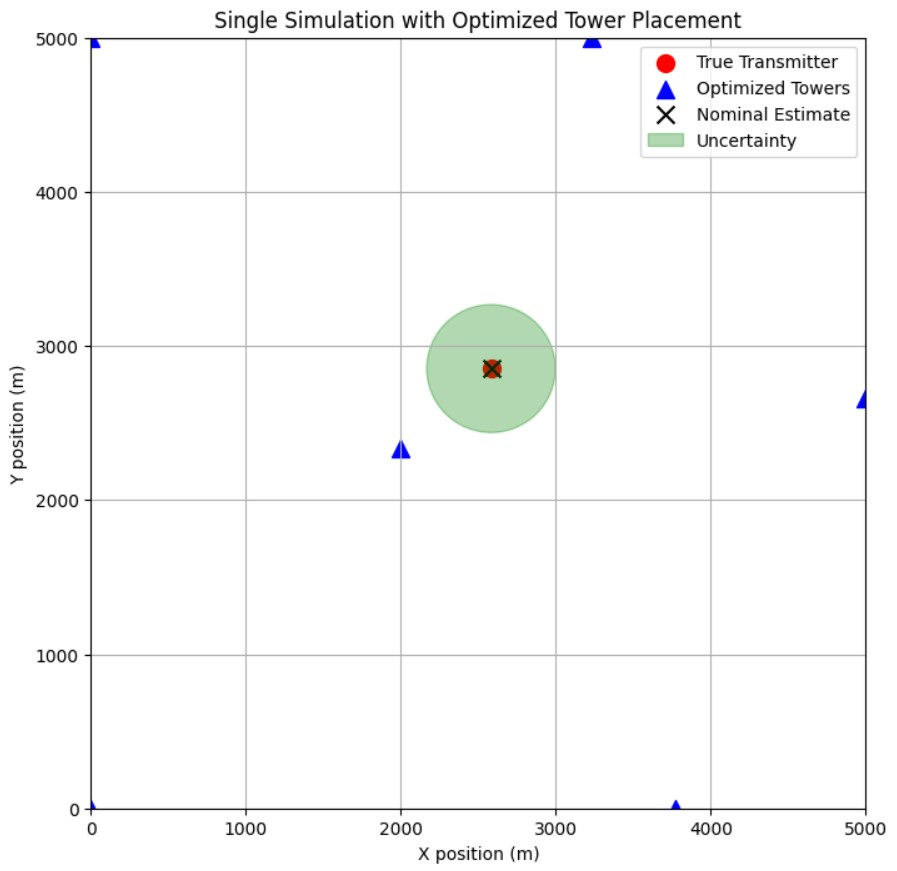
\includegraphics[width=\textwidth,keepaspectratio]{images/rtt/optimal_towers.jpg}
        \end{column}
    \end{columns}
    \vspace{0.5cm}
    \begin{itemize}
        \item Random Towers: Error = 59.77 ± 465.38 m, Radius = 1761.70 ± 2133.72 m
        \item Optimal Towers: Error = 0.00 ± 0.00 m, Radius = 550.41 ± 179.68 m
    \end{itemize}
\end{frame}


\begin{frame}{GPS vs. Time Accuracy Sensitivity}
    \centering
    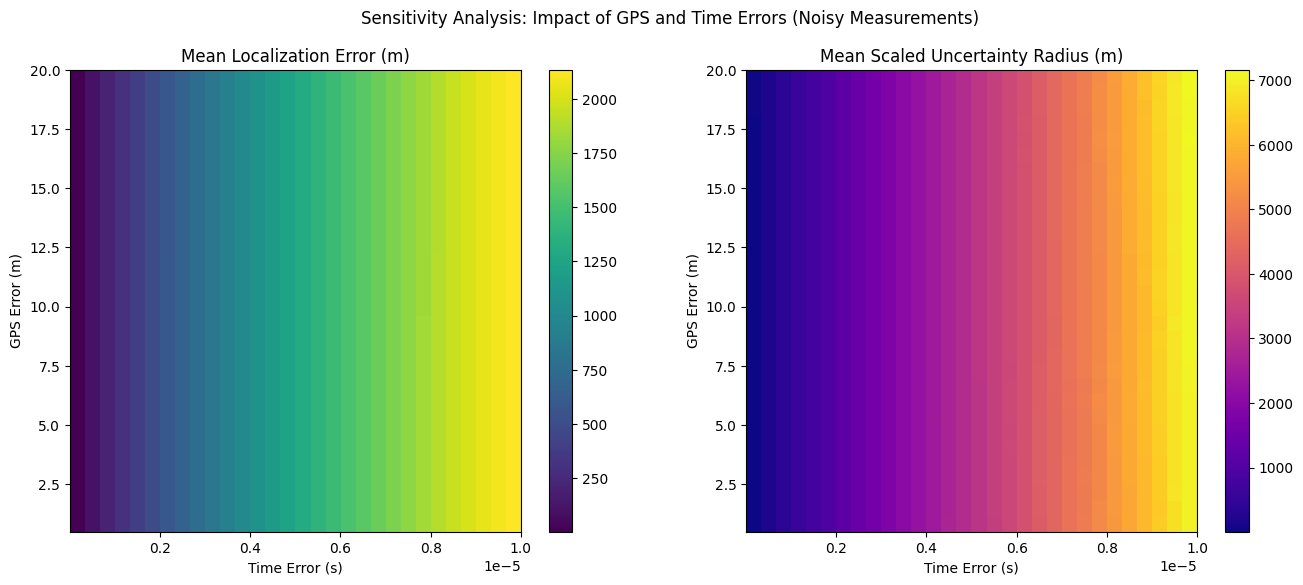
\includegraphics[height=0.7\textheight,width=0.7\textwidth,keepaspectratio]{images/rtt/gpstime.png}
    \vspace{0.5cm}
    \begin{itemize}
        \item Need for GPS-disciplined oscillator... possibly good enough GPS. 
    \end{itemize}
\end{frame}

\begin{frame}{USRP B200}
    \centering
    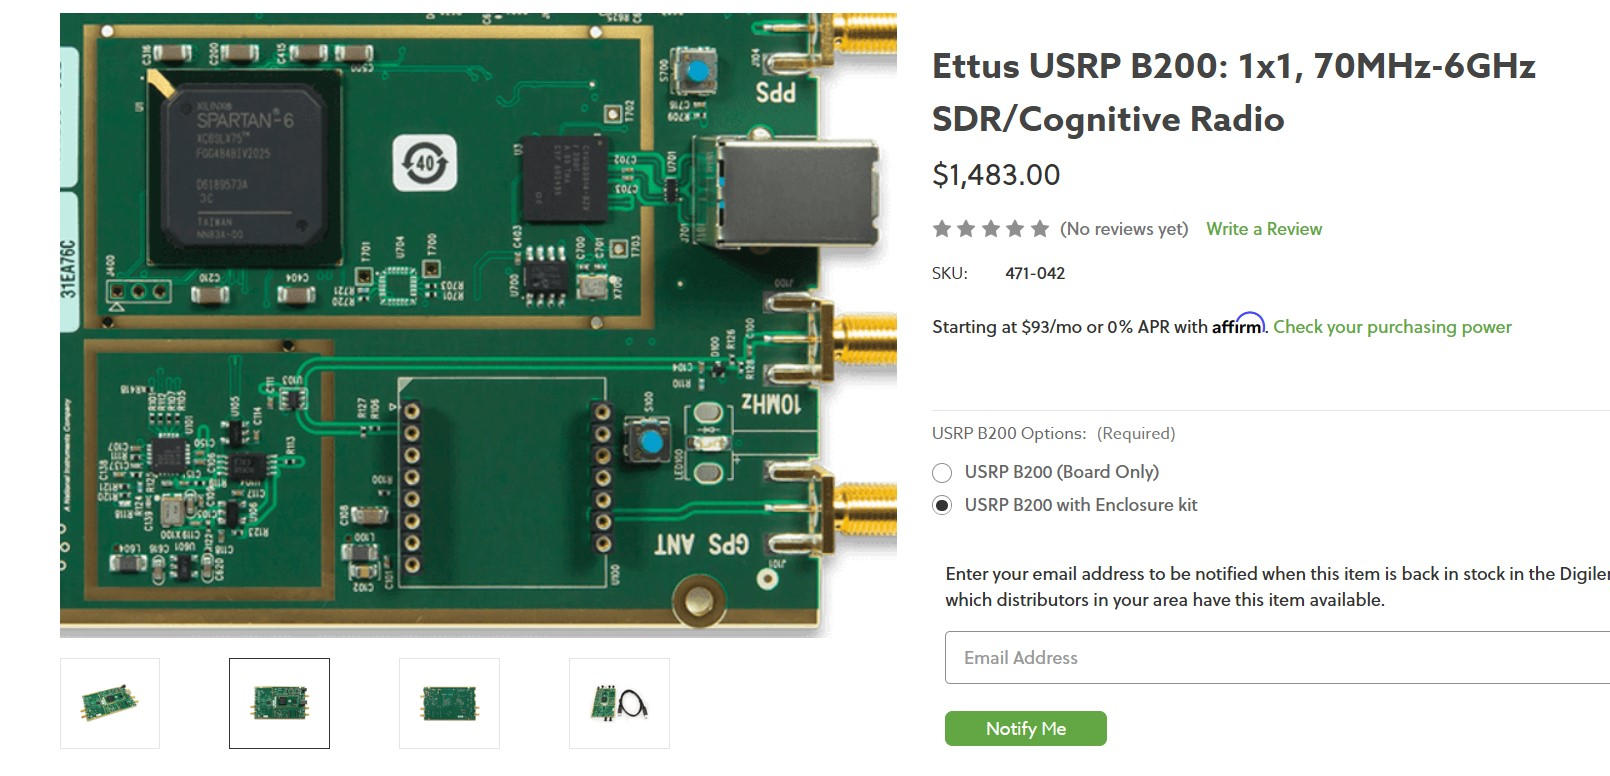
\includegraphics[height=0.7\textheight,width=0.7\textwidth,keepaspectratio]{images/rtt/usrp.jpg}
    \vspace{0.5cm}
    \begin{itemize}
        \item Takes care of GPSDO, GPS coordinates, and SDR.
    \end{itemize}
\end{frame}

\begin{frame}{ATLAS}
    \centering
    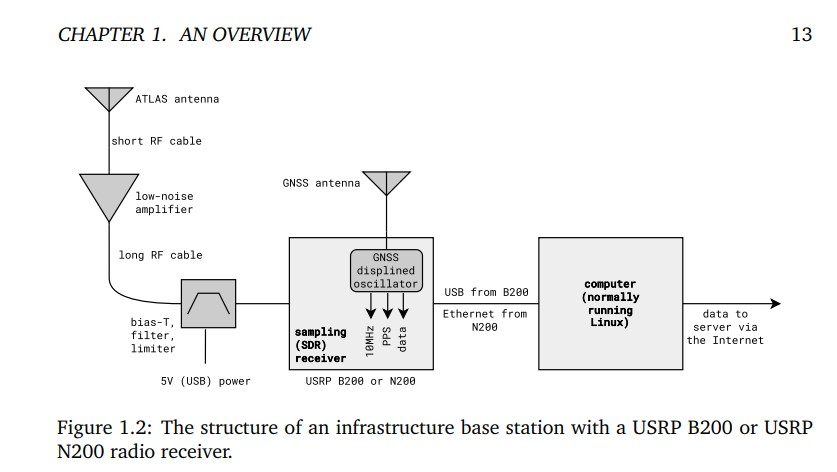
\includegraphics[height=0.7\textheight,width=0.7\textwidth,keepaspectratio]{images/rtt/atlas-hardware.jpg}
    \vspace{0.5cm}
    \begin{itemize}
        \item ATLAS is a TDOA localization system.
        \item Good reference for hardware/software design.
        \item Uses TCP/IP for communication and Vildehaye tags. 
    \end{itemize}
\end{frame}